\problemname{ETA}

You want to design a level for a computer game. The level can be described as
a connected undirected graph with vertices numbered from $1$ to $n$. In the game, the
player's character is dropped at one of the $n$ vertices uniformly at random
and their goal is to reach the exit located at vertex $1$ as quickly as
possible. Traversing an edge takes exactly $1$ second.

\begin{figure}[h]
	\centering
	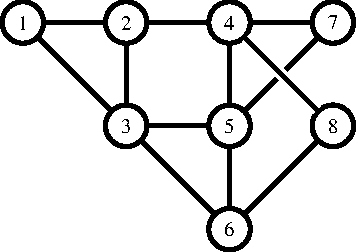
\includegraphics{sample}
	\caption{Illustration of Sample Output 3, a level where the average
	optimal time to reach vertex $1$ is $\frac{7}{4}$.}
  \label{fig:e}
\end{figure}

The difficulty of the level is determined by the average optimal time
to reach the exit. Given a target value for this average optimal time, construct a
level so that this target value is reached. See Figure~\ref{fig:e} for an example.

\begin{Input}
  The input consists of:
  \begin{itemize}
    \item One line with two coprime integers $a$ and $b$ ($1 \le a,b \le 1000$) separated by a
      `\texttt{/}', giving the desired average optimal time to reach the exit as the fraction $\frac{a}{b}$.
  \end{itemize}
\end{Input}

\begin{Output}
  If no connected graph with the average optimal time $\frac{a}{b}$ to reach vertex $1$ exists,
  output ``\texttt{impossible}''.
  Otherwise, output one such graph in the following format:
  \begin{itemize}
    \item Two integers $n$ and $m$ ($1 \le n, m \le 10^6$), the number
      of vertices and the number of edges.
    \item $m$ pairs of integers $u$ and $v$ ($1 \le u,v \le n$), indicating an edge between vertices $u$ and $v$.
  \end{itemize}
  The graph may include self loops and parallel edges.
  You are given that if there exists a valid graph, then there also exists one with $1 \le n, m \le 10^6$.

  If there are multiple valid solutions, you may output any one of them.
\end{Output}
